\documentclass[10pt]{article}
\usepackage[a4paper,margin=23mm]{geometry}
\usepackage[T1]{fontenc}
\usepackage{lmodern,amsmath,booktabs,longtable,graphicx,array,microtype}
\usepackage[colorlinks=true,urlcolor=blue,citecolor=blue,linkcolor=blue]{hyperref}
\usepackage[numbers,sort&compress]{natbib}
\usepackage[section]{placeins}
\usepackage{tikz}
\usetikzlibrary{arrows.meta,positioning}
\setlength{\parskip}{3pt}
\renewcommand{\topfraction}{.95}
\renewcommand{\bottomfraction}{.85}
\renewcommand{\textfraction}{.05}
\renewcommand{\floatpagefraction}{.6}
\setlength{\parindent}{1em}
\makeatletter
\setlength{\@fptop}{0pt}
\setlength{\@fpsep}{14pt}
\makeatother
\newcommand{\SURecall}{63.00\%}
\newcommand{\SUFone}{48.90\%}
\newcommand{\SUPrecision}{39.96\%}
\newcommand{\SURxFone}{48.90\%}
\newcommand{\SUSamples}{64,488}
\newcommand{\SUBytes}{655,648}
\newcommand{\SUFalse}{313}
\newcommand{\GateRecall}{48.83\%}
\newcommand{\GateFone}{40.58\%}
\newcommand{\GatePrecision}{34.72\%}
\newcommand{\GateRxFone}{40.61\%}
\newcommand{\GateSamples}{50,453}
\newcommand{\GateBytes}{1,113,522}
\newcommand{\GateFalse}{306}
\newcommand{\TrustRecall}{50.17\%}
\newcommand{\TrustFone}{38.32\%}
\newcommand{\TrustPrecision}{31.00\%}
\newcommand{\TrustRxFone}{38.34\%}
\newcommand{\TrustSamples}{67,222}
\newcommand{\TrustBytes}{1,169,204}
\newcommand{\TrustFalse}{447}
\newcommand{\DeltaThreshold}{2}
\newcommand{\VarianceThreshold}{2}
\newcommand{\RaoThreshold}{4}

\title{Trust-Aware Adaptive Sampling and Communication for Resource-Constrained IoT Monitoring: A Simulation-Based Evaluation}
\author{TAIS Research Project\\\small Author names and affiliations to be supplied before submission}
\date{Draft, 19 October 2026}
\begin{document}
\maketitle
\begin{abstract}
Single-node IoT monitoring must distinguish environmental events from sensor faults while limiting acquisition and transmission. We evaluate TAIS, an executable integration of heuristic sensor-health diagnostics, event-aware sampling, upload suppression, stateless binary snapshots, and an independently decoded receiver. Fixed-period, delta-driven, variance-driven, and explicitly Rao-inspired schedules provide independent controls. Evaluation uses two separately specified synthetic tasks: G1 supports development and held-out comparison, whereas G2 applies frozen policies without retuning and changes signal dynamics, fault processes, event timing, and ground-truth interval definitions. SU40's F1 difference from the variance-budget control changes from +4.88 percentage points in G1 to -4.32 in G2; the G2 descriptive seed-paired 95\% interval, [-9.11, +0.18], includes zero. Thus its near-budget quality advantage is not established across these tasks. Lower application-byte counts and fewer operationally attributed fault-induced reports coexist with missed short events and older receiver data. All communication counts come from actual encoding and independent receiver reconstruction. The study contributes reproducible system integration, independent resource comparisons, and explicit failure boundaries, rather than a new trust theory or universally superior policy. Two project-defined synthetic tasks and ideal local delivery do not establish field robustness or measured battery savings.

\end{abstract}

\section{Introduction}
Single-node IoT monitoring faces a three-way allocation problem: sparse sampling can miss environmental events, frequent observations can expose sensor artifacts, and transmission suppression can leave the receiver with old information. This matters in resource-constrained agricultural monitoring, but an application motivation does not itself provide evidence from agricultural deployments. The present study evaluates a two-channel software prototype under explicitly synthetic conditions.

Here, \emph{trust-aware} means that decisions use the heuristic state, flags and score supplied by SensorTrust C11. Trust is neither a calibrated fault probability nor a Bayesian reliability model, and it provides no formal guarantee of device trustworthiness. \emph{Resource cost} means software counts of sample cycles, uploads and encoded application bytes; it is not measured energy or battery lifetime. These definitions delimit the research question: \emph{what detection-quality, resource and information-age tradeoffs arise when health-aware sampling and upload rules operate under sensor faults, and which tradeoffs remain under two different synthetic task settings?}

Adaptive acquisition, fault-aware event decisions, predictive communication and their coordination already have substantial precedents \citep{rao2019adaptive,masoum2012quality,yim2010fault,dias2017dual,arnaiz2024energy}. The goal is therefore not to establish an optimal SU40 algorithm. The contributions are:
\begin{enumerate}
\item An executable integration of existing health diagnostics and change analysis with bounded sampling, explicit upload control, complete binary snapshots and independently decoded receiver evaluation.
\item A reproducible comparison against fixed-period, Delta, Variance and Rao-inspired schedules, separating native-system behavior, shared-detector diagnostics and actual nearby-budget qualification.
\item Evidence of conditional tradeoffs and failure boundaries across two synthetic tasks, including adverse independent-baseline comparisons, short-event misses, diagnostic blind spots and information-age costs.
\end{enumerate}
The second task changes event-label definitions as well as signal and fault processes. A contrast across these tasks cannot identify the effect of distribution change alone, and neither task validates real-field generalization.

\section{Related Work}
\paragraph{Adaptive acquisition.}
Rao et al. combine compressed sensing, prediction and switching around critical-sensing regions \citep{rao2019adaptive}. Masoum et al. study decentralized quality-aware sampling using correlation and prediction \citep{masoum2012quality}. DSRA adapts acquisition to signal changes within a self-adaptive software architecture \citep{algabroun2020dsra}. These precedents rule out claims that adaptation or its architectural integration originates here. Delta and Variance are independently implemented lightweight engineering controls, not reproductions of those papers.

\paragraph{Faults and environmental events.}
Sharma et al. evaluate fault-detection methods and fault prevalence in real deployment datasets \citep{sharma2010faults}; those data have a different evidential scope from our injected faults. Yim and Choi use neighboring readings and confidence for fault-tolerant event decisions \citep{yim2010fault}. CLARA uses cluster correlation for sampling adaptation and missing-reading reconstruction \citep{harb2024clara}. TAIS has no spatial reference or reconstruction of erased physical truth. Its C11 diagnostic rules and AdaptiveSense change analyzer are separately pinned software dependencies, not newly introduced fault classifiers.

\paragraph{Communication and joint control.}
Dual prediction reduces transmissions through synchronized models \citep{dias2017dual}, and relevance-aware monitoring coordinates acquisition and prediction under energy constraints \citep{arnaiz2024energy}. TAIS instead uses a last-sent deadband, heartbeat and explicit state edges, without a synchronized predictor, network optimizer or validated energy guarantee. The related-work artifact distinguishes detailed Rao-method inspection from abstract-level scope checks for other sources. No cross-paper performance numbers are treated as directly comparable results. Our Rao-inspired control omits compressed-sensing reconstruction and major prediction components; the original method's guarantees do not apply.

\section{System and Evaluation Interface}
\begin{figure}[tbp]\centering
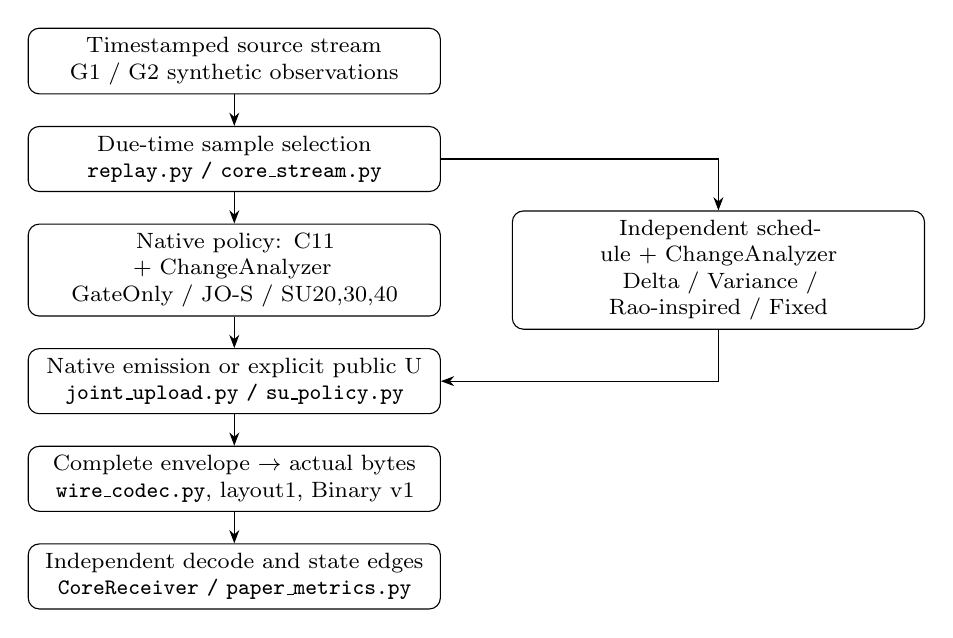
\begin{tikzpicture}[node distance=4mm,box/.style={draw,rounded corners,align=center,font=\footnotesize,text width=50mm,minimum height=8mm},>=Stealth]
\node[box] (input) {Timestamped source stream\\G1 / G2 synthetic observations};
\node[box,below=of input] (due) {Due-time sample selection\\\texttt{replay.py / core\_stream.py}};
\node[box,below=of due] (policy) {Native policy: C11 + ChangeAnalyzer\\GateOnly / JO-S / SU20,30,40};
\node[box,right=9mm of policy] (ind) {Independent schedule + ChangeAnalyzer\\Delta / Variance / Rao-inspired / Fixed};
\node[box,below=of policy] (up) {Native emission or explicit public U\\\texttt{joint\_upload.py / su\_policy.py}};
\node[box,below=of up] (wire) {Complete envelope $\to$ actual bytes\\\texttt{wire\_codec.py}, layout1, Binary v1};
\node[box,below=of wire] (rx) {Independent decode and state edges\\\texttt{CoreReceiver / paper\_metrics.py}};
\draw[->] (input)--(due);\draw[->] (due)--(policy);\draw[->] (due.east)-|(ind.north);
\draw[->] (policy)--(up);\draw[->] (ind.south)|-(up.east);\draw[->] (up)--(wire);\draw[->] (wire)--(rx);
\end{tikzpicture}
\caption{Implemented causal data path. The receiver observes decoded snapshots only. Independent +C11 versions attach diagnostics without health gating; optional U is an explicitly shared component. A separate G1 common-detector view preserves actual sample times and replaces only downstream detection and emission.}
\label{fig:architecture}
\end{figure}

The input contains timestamped temperature and humidity observations. Each policy reads values only when its sample is due; hidden generator parameters, event labels, faults and future observations are unavailable to decisions. SensorTrust C11 emits per-channel state, flags and score. AdaptiveSense supplies the original scheduler and ChangeAnalyzer. GateOnly applies health gating and recovery reseeding. JO-S adds bounded rechecks; JO-SU-20/30/40 retain that sampling design with different idle caps and attach upload module U. The historical default and prior NO-GO decisions are unchanged.

U compares a sampled value with the last transmitted snapshot, using a two-noise-floor deadband, a 120-second heartbeat evaluated at sample times, and emission on event, health state/flag and validity transitions. Score remains in every emitted health record, although a score-only change need not trigger transmission. Binary v1 retains timestamps, both values including null, event booleans and available health fields. Actual encoded length excludes hexadecimal log representation. Stateless frames decode independently; CRC checks accidental corruption, not authentication. The evaluated transport is ideal local delivery, without radio headers, loss, ACKs or retransmission.

Three outcome levels remain distinct. A \emph{local detection} is an active sampled episode; a \emph{sender report} is its first requested upload; a \emph{receiver report} is a false-to-true event transition reconstructed from decoded frames. A local clearing edge does not automatically reach the receiver. Exact sampled event and health transitions, including clears, are audited separately from environmental-event-to-report delays.

\section{Methods}
\subsection{Two synthetic tasks, including different truth definitions}
Both tasks supply 1,800 one-second source rows and separately retain latent physics, noisy pre-fault observations, faulted observations, event truth and fault schedules. All methods use identical instances within a task. The seven fault semantics are range, spike, stuck, drift, missing, invalid and stable offset. These are engineering stress distributions, not empirically fitted agricultural populations.

\paragraph{G1.}
The original mechanism uses a low-amplitude sinusoidal background, independent Gaussian noise and trapezoidal interventions with 26- or 180-second injected support. Physical-amplitude and duration rules determine interior event-label windows, which need not equal full injected support. Temperature carries the faults; same-channel events affect temperature and cross-channel events affect humidity. Event onset has a prescribed fault-relative delay. Three clean controls and seven fault kinds crossed with no/same/cross event arrangements and short/long profiles yield 45 scenarios. Development seeds 600--609 selected external operating points; final seeds 610--629 were evaluated after the committed freeze.

\paragraph{G2.}
The independently specified second mechanism uses piecewise random targets and a mean-reverting background,
\begin{equation}
b_{c,t}=b_{c,t-1}+0.003(\mu_{c,t}-b_{c,t-1})+s_cz_{c,t}.
\end{equation}
Target durations are 180--360 seconds. Hidden centers vary within 22--28$^\circ$C and 40--60\%RH; channel-innovation correlation changes between segments. Observation noise is AR(1), with coefficients 0.65--0.9, amplitude changes every 120 seconds and occasional Student-$t_3$ perturbations. Event-enabled channels receive short (12--40s), medium (41--100s) and long (101--240s) interventions with step/recovery, smooth or asymmetric shapes. Fault onset, duration, signed magnitude and recovery vary; both channels can be faulty. Drift integrates piecewise slopes, stuck retains the actual onset reading, and missing/invalid preserve their declared semantics. Event and fault schedules use independent SHA256-derived random streams; before/after/overlap relations are classified offline, not selected by detector outcomes.

G2 labels the \emph{complete exogenous support} $[t_0,t_0+d)$, represented on the source grid by inclusive window $[t_0,t_0+d-1]$. This is not G1's amplitude-defined interior window. Thus G1/G2 differ jointly in dynamics, noise, fault processes, event shapes, timing and \textbf{ground-truth interval definitions}. We compare within-task contrasts and their stability; we neither pool task outcomes nor attribute a contrast change to a single factor.

G2 includes four clean controls and seven fault kinds crossed with two faulty channels and no/same/cross event arrangements, yielding 46 scenarios. Engineering seeds 690/691 checked software only; the committed specification and analysis preceded final seeds 700--719. Fourteen frozen native systems were applied without retuning, generating the archived 12,880 system runs. G1 and G2 protocols, configuration, source hashes, complete schedules and all adverse instances remain available in the artifact. This revision uses stored outputs only and adds no simulation campaign.

\subsection{Controls, shared components and selection history}
Fixed5/10/20/30/40/60 reuse the original periodic replay, sample only due-time values and upload every sample. Delta responds to consecutive sampled amplitude and timestamp-normalized rate. Variance uses elapsed-time EWMA dispersion. Both increase sampling when their sampled statistic crosses a selected threshold and double the interval after sustained sampled stability, within fixed bounds. Rao-inspired uses at most four sampled points for linear trend/boundary prediction, with critical bands around fixed public priors and hysteresis. Its four-point fit is inspired by Rao's Eqs.~11--13, but it omits CS reconstruction, previous-day tolerance estimation, synchronized dual prediction and substitution of predictions for observations. All engineering departures are documented; this is \emph{not a faithful reproduction}.

Independent native schedules use the same sampled-only ChangeAnalyzer and every-sample emission. Explicit +C11 versions add unchanged diagnostics without affecting their schedules or event decisions. Selected +C11+U versions attach the public upload module as a diagnostic ablation. These extensions must not be mistaken for original external algorithms containing TAIS components. In G1, an additional common-detector view preserves each native sample schedule and applies identical downstream ChangeAnalyzer, metadata-only C11 and per-sample emission. It isolates sample-time consequences; native-system comparisons additionally contain gating, resets and upload effects.

G1 selected Delta/Variance thresholds from 2/4/8 and Rao-inspired thresholds from 4/8/12 at cap40 by development micro F1, then Recall, fewer samples and smaller threshold. An initial cap-only matching attempt failed; the retained, disclosed development refinement searched minimum intervals 10--35s and caps20--60s at the selected thresholds. Within the development qualification band, selection prioritized F1 and then closeness of sample totals. All fixed periods and original adaptive curve points remain in the held-out evidence. The final SU40-targeted controls use minimum/cap intervals of 10/50s (Delta), 10/60s (Variance) and 10/35s (Rao-inspired), with thresholds 2, 2 and 4 noise-floor units, respectively. G2 changes none of these choices: in particular, Rao-inspired retains 24$^\circ$C/45\%RH priors despite different hidden centers.

\subsection{Metrics and operational definitions}
The channel-aware one-to-one event matcher retains its 5-second tolerance. Precision, Recall and F1 use pooled TP/FP/FN within each task; no-event Recall is undefined, not zero. Local, sender and receiver counts remain separate. Coverage means at least one actual sample inside the truth support; covered-event success is conditional and does not replace Recall. Event delays exclude misses and are accompanied by FN and archived matched-in-both delay differences.

A \emph{fault-induced false report} is an operational attribution: an unmatched report on the fault channel during its fault or 120-second recovery window, without a coincident same-policy clean-counterfactual report within 5 seconds. The clean counterfactual preserves the exact physical sequence and noise, removing faults only; G2 cache identity hashes the full clean observations and labels. This statistic depends on attribution windows and matching tolerance and is not proof of strict physical causation. Health evaluation separately counts any raw C11 flag and the corresponding type bit. Stable offset has no dedicated C11 bit, so correct-type detection is N/A; another flag does not count as the right type.

Resource outcomes count actual sample cycles, uploads, $\sum\mathrm{len}(\mathrm{encode}(\mathrm{envelope}))$, and bytes/upload. Receiver age is current source time minus the timestamp of the latest decoded snapshot; null remains null. P95 pools all source-second age histograms rather than averaging per-run percentiles. Sampled-edge delivery and physical-event delay are different quantities.

\emph{Budget qualification} is an approximate count comparison, not exact equal-cost control. For target sample total $N_T$ and independent total $N_C$, the relative gap is
\begin{equation}
g=(N_C/N_T)-1,\qquad \text{qualified if } |g|\leq\epsilon.
\end{equation}
The original frozen rule used $\epsilon=0.05$ on actual totals. This revision's post-hoc sensitivity uses 0.02, 0.05 and 0.10 on the same saved points. It changes eligibility labels only, never parameters, samples or quality outcomes.

\subsection{Uncertainty and the status of the analyses}
Each task uses paired whole-seed bootstrap resampling (5,000 draws), retaining all scenarios of a resampled seed and recomputing micro rates. There are 20 final seed clusters per task; source seconds and scenario rows are not independent replicates. G1 and G2 use their separately frozen analysis seeds and are never combined for inference.

The repository protocols defined metric families, contrast lists, seed splits and the 5\% budget rule before their final runs. G1 development selection and the G2 no-retuning condition were likewise frozen. These are repository-frozen evaluation plans, not independently registered confirmatory trials or a design with one unique primary endpoint. Emphasizing F1, Variance and Fixed20 in the present narrative is a \emph{post-outcome editorial choice}. The fixed-point discussion and three-tolerance sensitivity are explicitly exploratory.

All reported intervals are pointwise, unadjusted, descriptive 95\% intervals. Many baselines, metrics and subgroups were examined. No family-wise error or false-discovery control is claimed; no new confirmatory test or adjusted $p$-value is retrofitted. An interval excluding zero describes that contrast under its seed-resampling assumptions and does not establish global superiority. An interval including zero establishes neither equivalence nor the direction of an overall effect.

\section{Results}
\subsection{Quality and resource tradeoffs within each task}
Table~\ref{tab:quality} places the same 14 native health-information systems side by side, keeping task-specific denominators separate. The full G1 native/common points, G2 receiver outcomes and adverse fault groups are in Appendices~\ref{app:complete}--\ref{app:diagnostics}. Figure~\ref{fig:quality} uses separate task panels and discrete markers; it does not depict a causal distribution-shift trajectory.
\begin{table}[tbp]\centering
\caption{Sender Precision, Recall and F1 (\%), separately for G1 and G2. All listed methods carry C11 information. B denotes the G1-selected SU40-targeted independent budget point, not guaranteed matching on G2. ``AS+C11'' is AdaptiveSense+TrustLog; ``Var'' is Variance. The full name Rao-inspired is retained.}
\begingroup\small\setlength{\tabcolsep}{4pt}\renewcommand{\arraystretch}{1.1}\begin{tabular}{lrrrrrr}\toprule
Mode & G1 P & G1 R & G1 F1 & G2 P & G2 R & G2 F1 \\\midrule
AS+C11 & 31.00 & 50.17 & 38.32 & 46.55 & 35.83 & 40.49 \\
Gate & 34.72 & 48.83 & 40.58 & 52.69 & 34.64 & 41.80 \\
Gate+U & 34.72 & 48.83 & 40.58 & 52.69 & 34.64 & 41.80 \\
SU20 & 43.06 & 71.83 & 53.84 & 64.33 & 66.30 & 65.30 \\
SU40 & 39.96 & 63.00 & 48.90 & 55.80 & 39.58 & 46.31 \\
Fixed-5 & 36.57 & 72.17 & 48.54 & 62.42 & 77.76 & 69.25 \\
Fixed-10 & 35.81 & 69.83 & 47.34 & 64.36 & 76.67 & 69.98 \\
Fixed-20 & 25.19 & 44.50 & 32.17 & 60.59 & 50.52 & 55.10 \\
Fixed-30 & 22.12 & 35.17 & 27.16 & 54.72 & 38.65 & 45.30 \\
Fixed-40 & 28.40 & 42.50 & 34.05 & 49.24 & 23.70 & 32.00 \\
Fixed-60 & 31.06 & 43.17 & 36.12 & 41.39 & 15.52 & 22.58 \\
Delta-B & 36.11 & 63.67 & 46.08 & 61.44 & 65.57 & 63.44 \\
Var-B & 34.71 & 60.17 & 44.02 & 53.34 & 48.18 & 50.63 \\
Rao-inspired-B & 35.90 & 63.00 & 45.74 & 64.21 & 75.68 & 69.47 \\
\bottomrule\end{tabular}\endgroup
\label{tab:quality}
\end{table}
\begin{figure}[tbp]\centering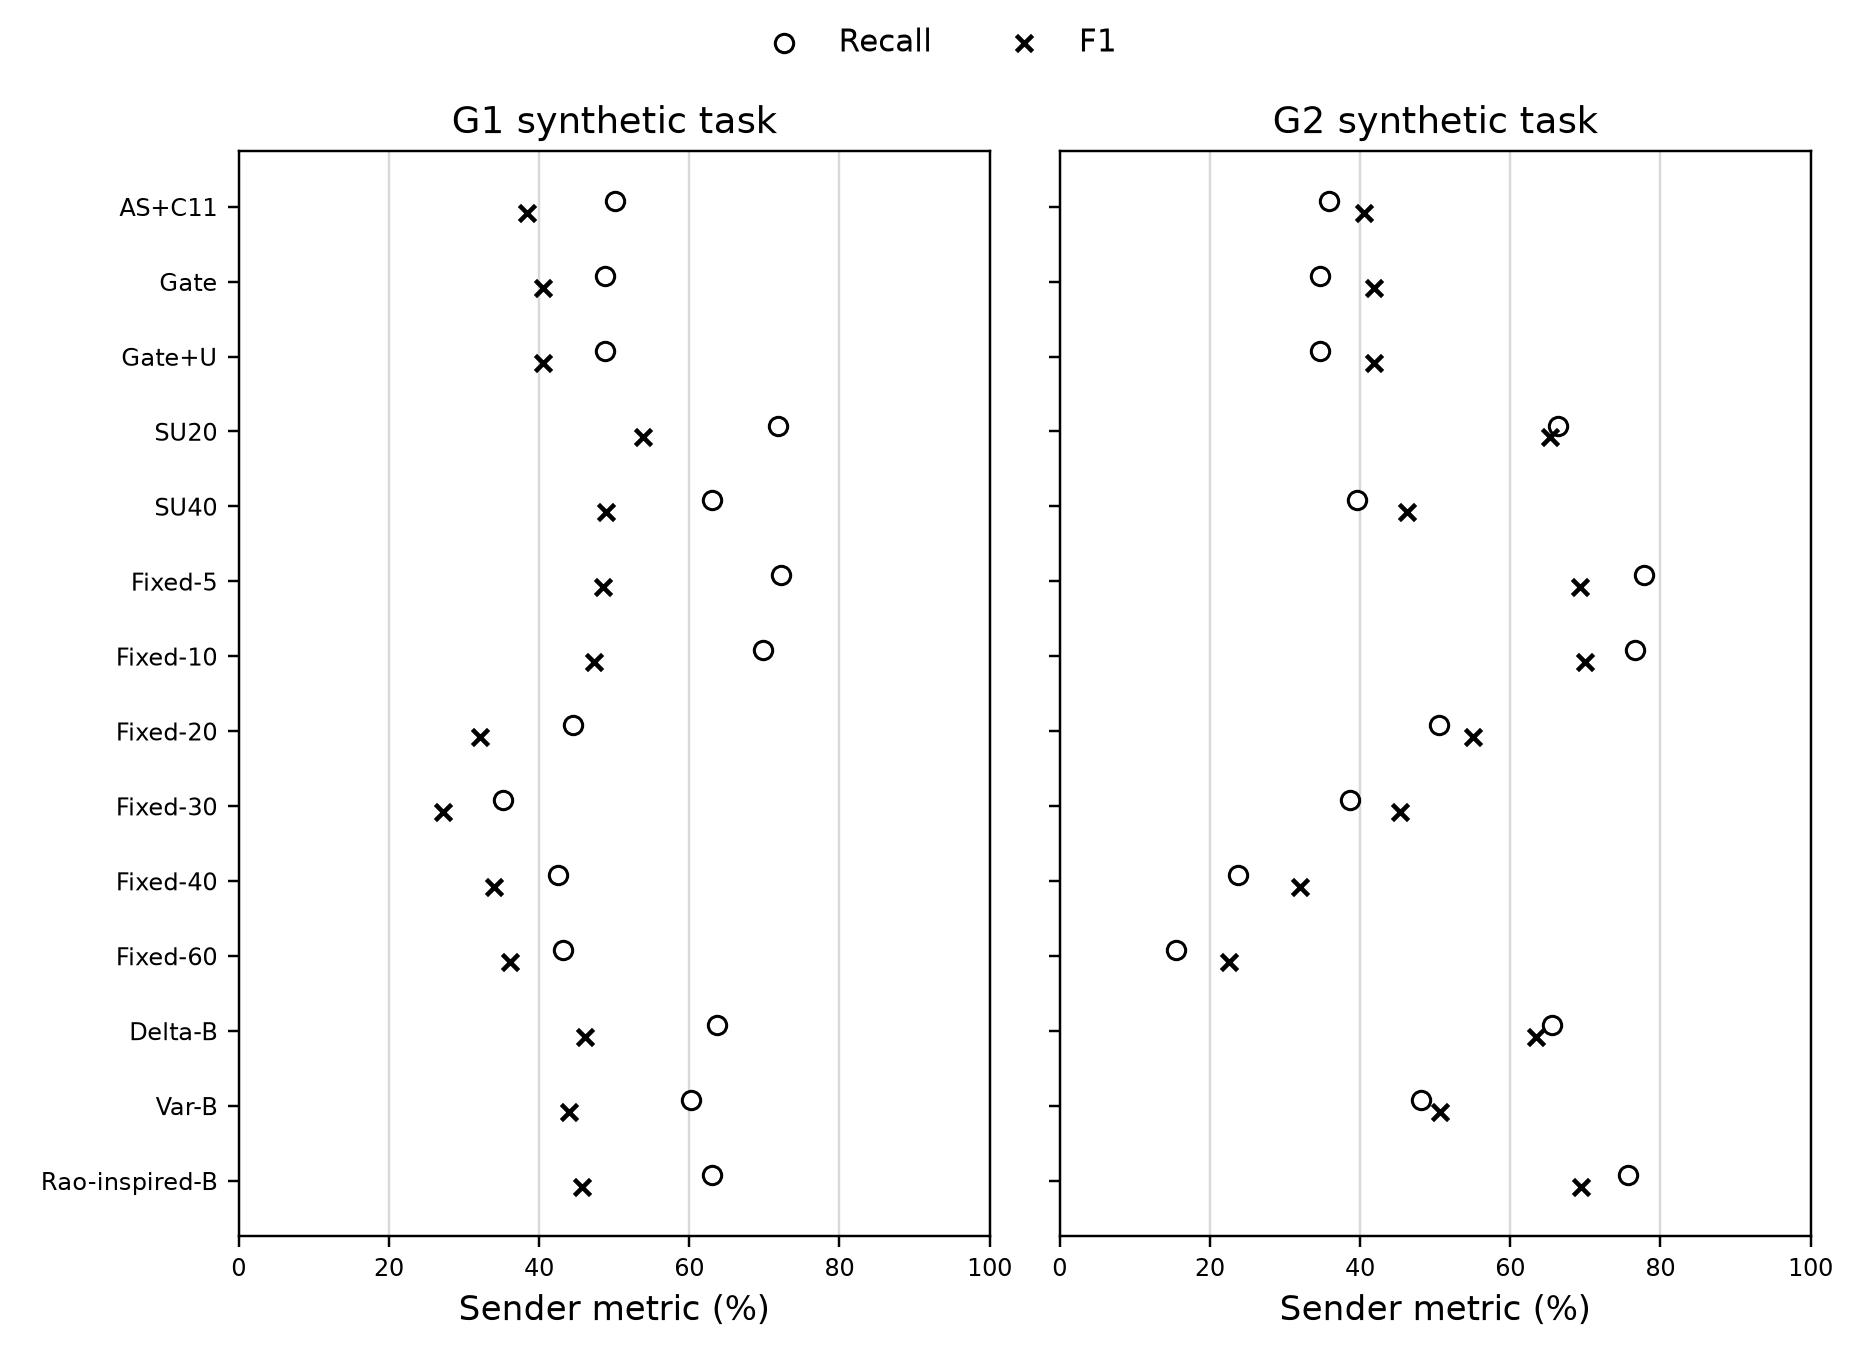
\includegraphics[width=\linewidth]{figures/review_task_quality.png}
\caption{Discrete sender quality under two different synthetic tasks. Open circles denote Recall and crosses denote F1, distinguishable in grayscale. Methods and parameters are frozen, but signal/fault/timing and truth definitions differ. Absolute task rates are not pooled or interpreted as an isolated distribution effect.}\label{fig:quality}
\end{figure}
In G1, SU40-minus-Variance F1 is +4.88 percentage points (pp), with pointwise interval [+0.82, +8.84]. In G2, the corresponding difference is -4.32 pp, interval [-9.11, +0.18]. This interval includes zero: it does not establish either an F1 advantage for SU40 or an overall F1 disadvantage. The G2 Recall difference is -8.59 pp, interval [-14.58, -2.97], which lies below zero descriptively. These are unadjusted, endpoint-specific intervals, not a multiple-comparison-controlled superiority test.

SU20 reaches G2 Recall 66.30\% and F1 65.30\%; SU40 reaches 39.58\% and 46.31\%. This difference comes with 43.84\% more sample cycles and FI counts 193 versus 157. It is a different operating tradeoff, not a universally improved setting. Independent controls remain competitive: G2's higher-quality Delta and Rao-inspired budget points have sample gaps +41.77\% and +88.08\%, so they do not qualify as nearby-budget comparisons at any displayed tolerance.


\subsection{Actual acquisition budgets and receiver age}
Table~\ref{tab:resources} reports measured software counts and original-rule qualification. A gap compares the displayed method with SU40 \emph{within the same task}; identical labels do not imply identical counts across tasks. Counts across G1/G2 should not be ratioed as if event/fault mixtures were the same. GateOnly+U remains a lower-cost option with the same sender quality as GateOnly; no mode is removed for being competitive.
\begin{table}[htbp]\centering
\caption{Native software resource counts, operationally attributed FI reports, pooled P95 source-data age and sample-gap qualification relative to each task's SU40. A ``yes'' marks $|g|\leq5\%$, not exact equal budgets. Fixed periods and all three independent budget controls are retained. Upload counts, mean bytes/upload and maximum age remain in the appendix/artifact.}
\begingroup\small\setlength{\tabcolsep}{4pt}\renewcommand{\arraystretch}{1.1}\begin{tabular}{lrrrrrr}\toprule
Mode & Samples & Bytes & FI & Age P95(s) & Gap(\%) & 5\% \\\midrule
\multicolumn{7}{l}{\textit{G1: separate task totals}} \\
AS+C11 & 67,222 & 1,169,204 & 447 & 57 & +4.24 & yes \\
Gate & 50,453 & 1,113,522 & 306 & 58 & -21.76 & no \\
Gate+U & 50,453 & 617,988 & 306 & 115 & -21.76 & no \\
SU20 & 100,810 & 699,046 & 319 & 113 & +56.32 & no \\
SU40 & 64,488 & 655,648 & 313 & 113 & +0.00 & yes \\
Fixed-5 & 324,000 & 11,418,840 & 540 & 4 & +402.42 & no \\
Fixed-10 & 162,000 & 5,709,420 & 551 & 9 & +151.21 & no \\
Fixed-20 & 81,000 & 2,854,260 & 441 & 18 & +25.60 & no \\
Fixed-30 & 54,000 & 1,902,540 & 418 & 28 & -16.26 & no \\
Fixed-40 & 40,500 & 1,426,680 & 385 & 37 & -37.20 & no \\
Fixed-60 & 27,000 & 950,820 & 371 & 56 & -58.13 & no \\
Delta-B & 70,584 & 2,474,326 & 467 & 45 & +9.45 & no \\
Var-B & 63,391 & 2,206,528 & 454 & 55 & -1.70 & yes \\
Rao-inspired-B & 65,510 & 2,282,729 & 466 & 32 & +1.58 & yes \\
\multicolumn{7}{l}{\textit{G2: separate task totals}} \\
AS+C11 & 81,474 & 1,392,252 & 339 & 58 & -4.21 & yes \\
Gate & 70,542 & 1,347,319 & 137 & 58 & -17.06 & no \\
Gate+U & 70,542 & 858,092 & 137 & 116 & -17.06 & no \\
SU20 & 122,343 & 1,154,911 & 193 & 110 & +43.84 & no \\
SU40 & 85,055 & 959,129 & 157 & 113 & +0.00 & yes \\
Fixed-5 & 331,200 & 11,764,583 & 490 & 4 & +289.40 & no \\
Fixed-10 & 165,600 & 5,882,392 & 424 & 9 & +94.70 & no \\
Fixed-20 & 82,800 & 2,940,838 & 353 & 18 & -2.65 & yes \\
Fixed-30 & 55,200 & 1,960,460 & 315 & 28 & -35.10 & no \\
Fixed-40 & 41,400 & 1,470,061 & 277 & 37 & -51.33 & no \\
Fixed-60 & 27,600 & 979,596 & 217 & 56 & -67.55 & no \\
Delta-B & 120,579 & 4,286,926 & 371 & 39 & +41.77 & no \\
Var-B & 84,429 & 2,989,505 & 361 & 53 & -0.74 & yes \\
Rao-inspired-B & 159,972 & 5,683,495 & 418 & 9 & +88.08 & no \\
\bottomrule\end{tabular}\endgroup
\label{tab:resources}
\end{table}

The complete post-hoc sensitivity table (Appendix~\ref{app:sensitivity}) includes all existing independent +C11 native control--target pairs at 2\%, 5\% and 10\%. Five percent reproduces the historical rule; the three-way sensitivity analysis itself is new and post hoc. Threshold changes qualify or disqualify some existing comparisons without changing any performance value. In particular, fixed-period and development-named controls are not reselected to obtain a favorable match.
The receiver is evaluated from decoded frames, not copied sender state. In G2, SU40 receiver TP/FP/FN are 760/602/1,160, with 0 missed sampled event/health edges. GateOnly misses 2 sampled edges; Gate+U misses 0. Restoring edges can also expose a false onset, so exact delivery is not synonymous with higher event F1. Detailed local/sender/receiver counts and conditional delays remain in the appendix and artifact.


\subsection{Failure boundaries}
In G2, SU20 covers 92.34\% of short events but reports only 37.34\%; SU40 reports 9.22\%, versus GateOnly's 9.69\%. Coverage therefore does not guarantee that confirmation, gating and event shape permit a report. GateOnly, SU20 and SU40 each miss all 52 full-support replacement events. Some independent-method reports can coincide with these labels; such coincidences do not establish reconstruction of erased physical information. SU40 stable-offset any-flag detection is 5.83\%; a correct offset type is unsupported because C11 has no dedicated offset bit. Humidity-fault Recall is 38.10\%, so adding the second faulty channel does not remove missed-event limitations.

Raw health detection also depends on when the frozen C11 rule receives observations. A sampled flag need not identify the physical cause, and conditional flag delays omit undetected episodes. Full-support replacement and no-sample coverage are retained in all overall denominators; finite-valued coverage is separately archived. These findings delimit the information available to a single node, rather than validating recovery of hidden events.

\section{Discussion}
\subsection{What the G1/G2 comparison establishes}
SU40's near-budget detection-quality advantage observed in G1 was not retained under the independently specified G2 synthetic task, which differs in signal dynamics, fault processes, event timing, and ground-truth interval definitions. The experiment cannot separately identify the contributions of distributional changes, pulse shapes, or label geometry. In particular, comparing absolute G1/G2 Recall as if only the input distribution changed would be misleading. The G2 F1 point estimate favors Variance (50.63\% versus 46.31\%), but its interval includes zero; the narrower defensible conclusion is absence of support for SU40's nearby-budget F1 advantage in this task.

Both tasks were specified within this project. Their differences provide a useful stress test of a broad superiority claim, but do not isolate the causes of a changed contrast or simulate an external-field validation. The lower Recall interval against Variance must be read as one descriptive endpoint among many, alongside the F1 interval spanning zero. Likewise, Fixed20's higher observed F1 is important adverse evidence, not a new confirmatory global ranking.

\subsection{Fixed20 versus SU40: conflicting objectives}
Fixed20+C11 makes the objective conflict concrete. On G2 its F1 is 55.10\%, compared with SU40's 46.31\%, while sample totals are 82,800 and 85,055, respectively. The control's relative sample gap is -2.65\%, within the original qualification band. These are descriptive point comparisons, not evidence of a stable global Fixed20 advantage. SU40 emits 959,129 rather than 2,940,838 application bytes and has 157 rather than 353 operationally attributed fault-induced reports. Its pooled P95 age is 113 rather than 18s. Thus better quality at similar acquisition counts coexists with more communication and more attributed reports, while suppression coexists with substantially older ordinary data. Neither mode dominates these dimensions.

\begin{figure}[tbp]\centering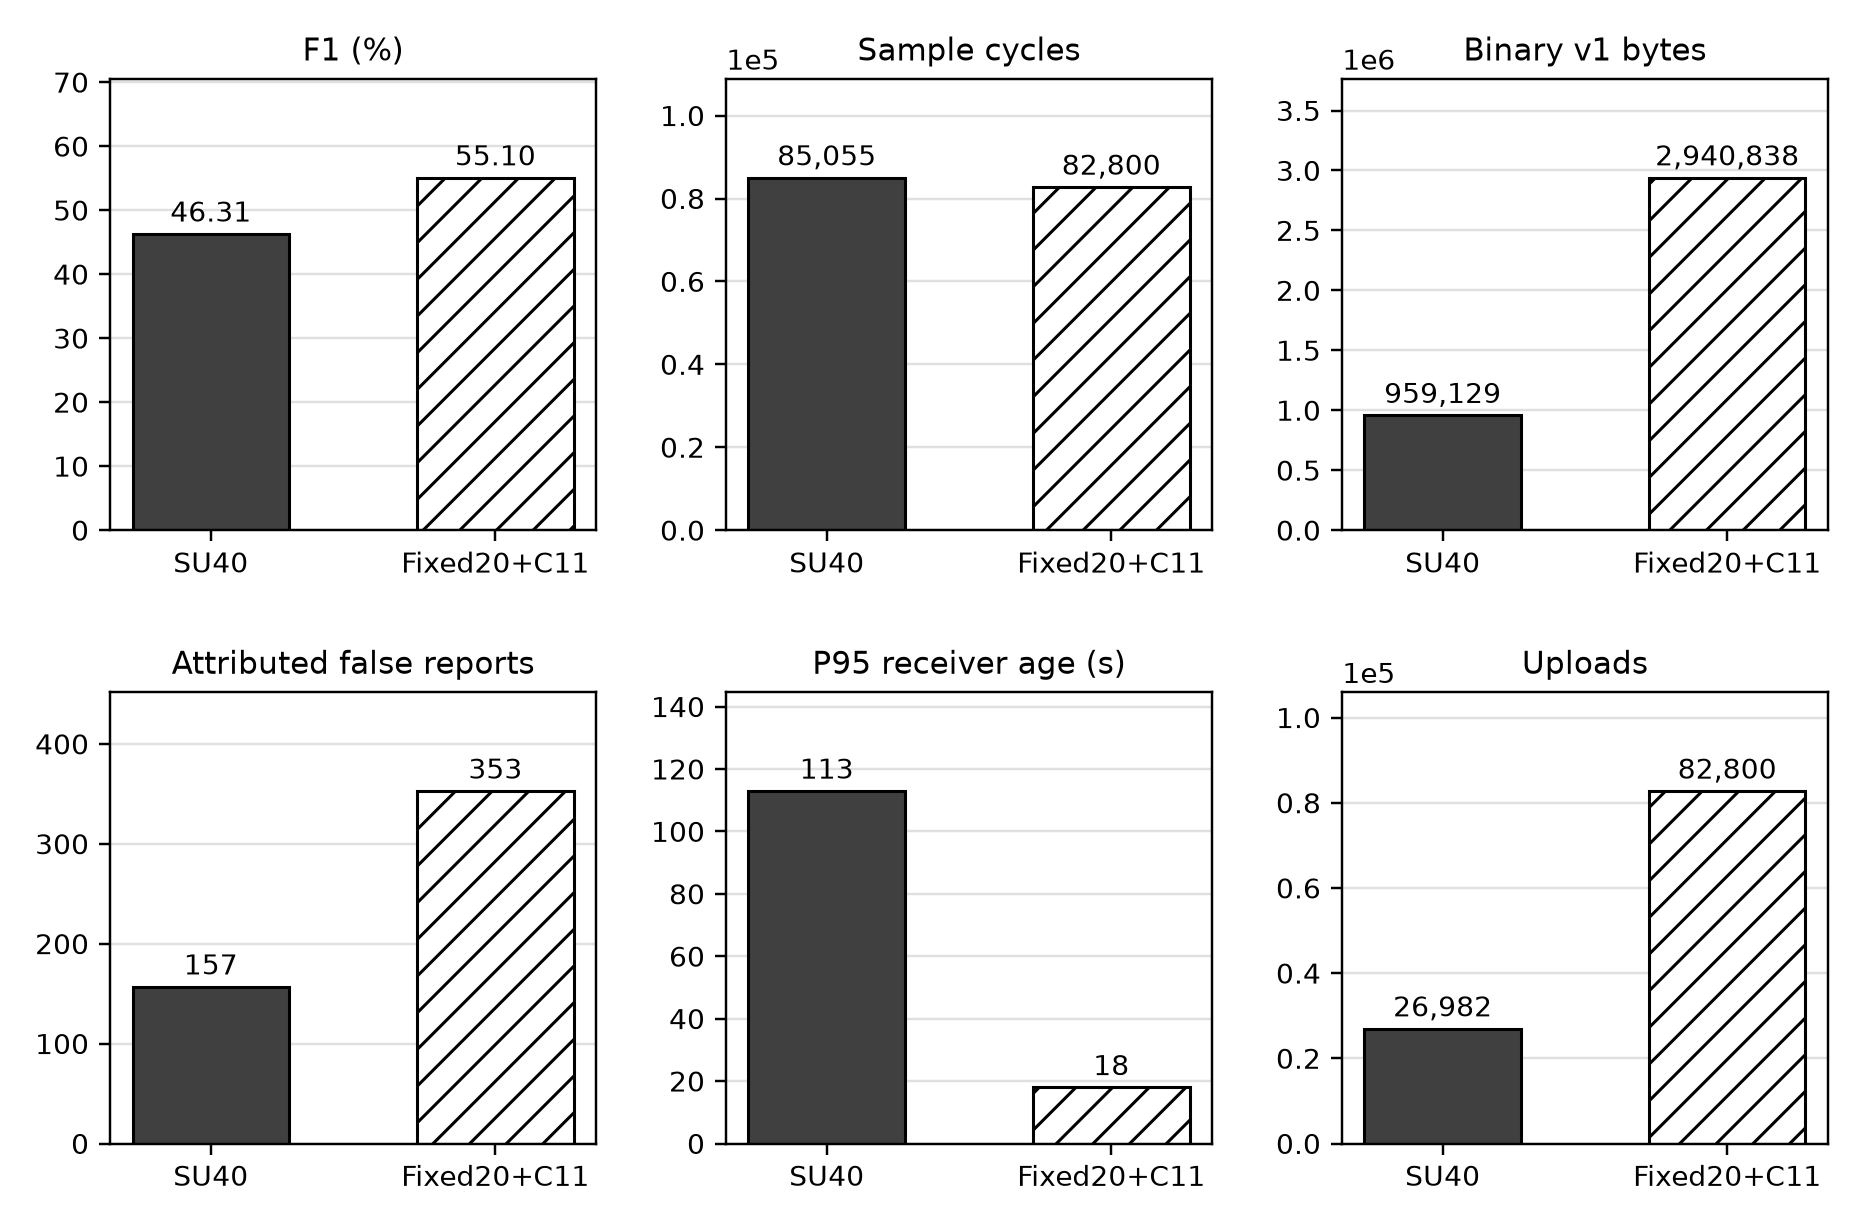
\includegraphics[width=\linewidth]{figures/review_fixed20_tradeoff.png}
\caption{G2 tradeoff at nearby acquisition totals: filled bars are SU40 and hatched bars Fixed20+C11. Panels show actual values on their own scales; higher is preferable for F1, whereas other objectives depend on the application's cost and freshness requirements. No single aggregated utility or hardware-energy model is imposed.}\label{fig:fixedtradeoff}
\end{figure}
On G2, GateOnly and Gate+U have identical sender quality and 70,542 sample cycles, but bytes change from 1,347,319 to 858,092, and pooled P95 age from 58 to 116s. The G1 independent-schedule +U ablations likewise retain schedules and sender reports (Appendix~\ref{app:diagnostics}). Consequently, communication savings are partly attributable to a reusable upload rule; they cannot all be credited to the originality of SU40 sampling. The G1 common-detector view isolates sample schedules, whereas native comparisons also include gating, reset and emission behavior.

Accordingly, the native comparison measures complete system choices, not the isolated originality of a sampling rule. A deployment selecting a mode would need to specify acceptable misses, attributed false reports, age and transmission overhead. The data do not supply a universal weighting or an optimal default.

\subsection{Implications of the negative cases}
More samples can expose an event often enough to confirm it, but can also expose additional sensor artifacts. The historical H layer illustrates the risk of treating a slow trend as fault evidence: it lost true events and added other false reports. Its NO-GO finding and the unchanged historical default remain part of the research record; they are not new successful contributions. Stable offsets, slow physical changes and drift can remain ambiguous without independent references. Sampling cannot restore values overwritten by a fault or events never observed between samples.

Communication suppression addresses a different objective. The measured byte reduction is useful software evidence, but it excludes packet headers, receive windows, airtime, modulation, contention and retries. Even an additive model $C=aN_{\rm sample}+bN_{\rm upload}+B+P$ is conditional on weights and processing cost. The archived dimensionless sensitivity grid assumes equal processing when comparing ratios; it is not a measured joule model. In particular, byte ratios cannot establish equal energy ratios or battery-life gains.

\section{Limitations and Threats to Validity}
\paragraph{Task validity and identifiability.}
The evidence consists of two project-defined synthetic tasks, not natural-fault or agricultural-event ground truth. G1 has temperature-only faults and prescribed timing; G2 broadens mechanisms and faulty channels but changes label geometry too. These factors are confounded, so no individual shift effect is identified. The source distributions, amplitudes, timing strata and pulse definitions may favor particular detector behaviors. No claim of representativeness or external-field robustness follows.

\paragraph{Comparison and statistical validity.}
Independent schedules share an external event analyzer; metadata extensions and public U variants are explicitly distinguished. Delta and Variance are simple engineering controls, and Rao-inspired is an incomplete adaptation rather than a faithful full-method benchmark. G1 development searches constrain generality; seed-bootstrap intervals do not account for model misspecification, developer choices or all selection effects. Numerous unadjusted endpoints and post-outcome editorial emphasis prohibit confirmatory global superiority claims. Budget qualification depends on tolerance and total counts, not identical per-scenario acquisition opportunities.

\paragraph{Transport, hardware and measurement validity.}
Local ideal delivery omits real wireless behavior. There are no MCU timing/RAM benchmarks, measured currents, energy coefficients or battery trials. A sample cycle is a processing opportunity, not measured sensor power gating. A fresh timestamp may contain null and is not equivalent to accurate usable data. Conditional delays exclude misses; fault-induced attribution and event matching depend on the declared windows. Full-support replacement marks overwritten dynamic support; a stuck onset reading can still contain prior physical information. No calibrated reliability probability or guarantee of recovering erased events is offered.

\section{Conclusion}
TAIS provides an auditable integration for examining quality, acquisition, transmission and receiver-age tradeoffs under sensor faults. Independent controls, actual budget qualification and decoded receiver checks prevent a favorable internal comparison from becoming a universal-optimality claim. The nearby-budget F1 advantage observed in G1 is not established under the differently defined G2 task; its F1 point estimate favors Variance while the interval includes zero. Fixed20 also exposes a quality-versus-communication tradeoff at similar sample totals. The defensible contribution is reproducible systems evaluation with explicit negative evidence and failure boundaries. These simulation results support conditional design analysis, not a new trust theory, field validation or measured energy savings.

\section*{Artifact, attribution and AI-use disclosure}
The revision and complete frozen evidence are at \href{https://github.com/Sver0411/TAIS/tree/docs/tais-paper-major-revision}{the TAIS revision artifact repository}. AdaptiveSense commit\texttt{f7ec30fd} and SensorTrust commit\texttt{2ce98dd0} are unmodified, separately attributed MIT-licensed components. Original G1/G2 results, protocols and negative conclusions remain unchanged. Tables and plots are generated from frozen CSVs with source/cell audits; compressed traces are enumerated by hashes and deterministically reproducible. This paper revision adds only read-only budget sensitivity and presentation changes, not new simulation outcomes.

\textit{Draft disclosure for author verification:} OpenAI Codex assisted implementation, analysis scripting, checking and manuscript preparation. Figures are deterministic plots of saved numerical outputs or a code-based architecture diagram. Human authors must independently review the outputs, confirm the precise tool-use scope and approve the submission; this draft does not assert that such approval has occurred. The final disclosure location and wording must follow the selected venue's current rules. Author identities, affiliations and funding have not been supplied and are not invented here.
\bibliographystyle{unsrtnat}
\bibliography{references}
\clearpage
\appendix
\section{Complete operating points and comparison views}\label{app:complete}
All G1 native points below are retained, including health-free payloads (functionally unequal), +C11 metadata versions, +U diagnostics and budget points. P/R/F1 and receiver F1 are percentages; all source scenarios and final seeds are retained. SU abbreviates JO-SU; S denotes JO-S; G/B denote points targeted during G1 development to GateOnly/SU40, not guarantees of final equality. Complete per-run, fault, channel, duration, timing and no-event groups are linked from the artifact evidence report.
\subsection{G1 native systems}
\begin{scriptsize}\setlength{\tabcolsep}{3pt}\begin{longtable}{lrrrrrrr}
\toprule Method & P & R & F1 & RxF1 & Samples & Bytes & FI \\\midrule\endhead
AS & 31.00 & 50.17 & 38.32 & 38.34 & 67,222 & 969,950 & 447 \\
AS+C11 & 31.00 & 50.17 & 38.32 & 38.34 & 67,222 & 1,169,204 & 447 \\
Delta-bGate & 34.02 & 58.00 & 42.88 & 42.88 & 51,070 & 1,486,276 & 441 \\
Delta-bGate+C11 & 34.02 & 58.00 & 42.88 & 42.88 & 51,070 & 1,792,696 & 441 \\
Delta-bS40 & 36.11 & 63.67 & 46.08 & 46.08 & 70,584 & 2,050,822 & 467 \\
Delta-bS40+C11 & 36.11 & 63.67 & 46.08 & 46.08 & 70,584 & 2,474,326 & 467 \\
Delta-20 & 37.73 & 71.50 & 49.40 & 49.40 & 239,766 & 6,970,632 & 477 \\
Delta-20+C11 & 37.73 & 71.50 & 49.40 & 49.40 & 239,766 & 8,409,228 & 477 \\
Delta-40 & 36.94 & 68.83 & 48.08 & 48.08 & 215,098 & 6,238,198 & 477 \\
Delta-40+C11 & 36.94 & 68.83 & 48.08 & 48.08 & 215,098 & 7,528,786 & 477 \\
Delta-40+C11+U & 36.94 & 68.83 & 48.08 & 48.08 & 215,098 & 778,846 & 477 \\
Delta-60 & 34.90 & 63.00 & 44.92 & 44.92 & 188,337 & 5,443,733 & 472 \\
Delta-60+C11 & 34.90 & 63.00 & 44.92 & 44.92 & 188,337 & 6,573,755 & 472 \\
Fixed-10 & 35.81 & 69.83 & 47.34 & 47.34 & 162,000 & 4,737,420 & 551 \\
Fixed-10+C11 & 35.81 & 69.83 & 47.34 & 47.34 & 162,000 & 5,709,420 & 551 \\
Fixed-20 & 25.19 & 44.50 & 32.17 & 32.17 & 81,000 & 2,368,260 & 441 \\
Fixed-20+C11 & 25.19 & 44.50 & 32.17 & 32.17 & 81,000 & 2,854,260 & 441 \\
Fixed-30 & 22.12 & 35.17 & 27.16 & 27.16 & 54,000 & 1,578,540 & 418 \\
Fixed-30+C11 & 22.12 & 35.17 & 27.16 & 27.16 & 54,000 & 1,902,540 & 418 \\
Fixed-40 & 28.40 & 42.50 & 34.05 & 34.05 & 40,500 & 1,183,680 & 385 \\
Fixed-40+C11 & 28.40 & 42.50 & 34.05 & 34.05 & 40,500 & 1,426,680 & 385 \\
Fixed-5 & 36.57 & 72.17 & 48.54 & 48.54 & 324,000 & 9,474,840 & 540 \\
Fixed-5+C11 & 36.57 & 72.17 & 48.54 & 48.54 & 324,000 & 11,418,840 & 540 \\
Fixed-60 & 31.06 & 43.17 & 36.12 & 36.12 & 27,000 & 788,820 & 371 \\
Fixed-60+C11 & 31.06 & 43.17 & 36.12 & 36.12 & 27,000 & 950,820 & 371 \\
Gate & 34.72 & 48.83 & 40.58 & 40.61 & 50,453 & 1,113,522 & 306 \\
Gate+U & 34.72 & 48.83 & 40.58 & 40.58 & 50,453 & 617,988 & 306 \\
S & 43.06 & 71.83 & 53.84 & 53.84 & 100,810 & 1,241,098 & 319 \\
SU20 & 43.06 & 71.83 & 53.84 & 53.84 & 100,810 & 699,046 & 319 \\
SU30 & 39.10 & 61.00 & 47.66 & 47.66 & 76,736 & 665,780 & 316 \\
SU40 & 39.96 & 63.00 & 48.90 & 48.90 & 64,488 & 655,648 & 313 \\
Rao-bGate & 34.45 & 60.17 & 43.81 & 43.81 & 50,105 & 1,432,818 & 462 \\
Rao-bGate+C11 & 34.45 & 60.17 & 43.81 & 43.81 & 50,105 & 1,733,448 & 462 \\
Rao-bS40 & 35.90 & 63.00 & 45.74 & 45.74 & 65,510 & 1,889,669 & 466 \\
Rao-bS40+C11 & 35.90 & 63.00 & 45.74 & 45.74 & 65,510 & 2,282,729 & 466 \\
Rao-20 & 37.79 & 71.67 & 49.48 & 49.48 & 120,666 & 3,473,344 & 467 \\
Rao-20+C11 & 37.79 & 71.67 & 49.48 & 49.48 & 120,666 & 4,197,340 & 467 \\
Rao-40 & 35.96 & 67.00 & 46.80 & 46.80 & 106,051 & 3,038,490 & 470 \\
Rao-40+C11 & 35.96 & 67.00 & 46.80 & 46.80 & 106,051 & 3,674,796 & 470 \\
Rao-40+C11+U & 35.96 & 67.00 & 46.80 & 46.80 & 106,051 & 732,144 & 470 \\
Rao-60 & 33.92 & 60.67 & 43.51 & 43.51 & 156,591 & 4,527,190 & 468 \\
Rao-60+C11 & 33.92 & 60.67 & 43.51 & 43.51 & 156,591 & 5,466,736 & 468 \\
Var-bGate & 31.34 & 53.33 & 39.48 & 39.48 & 52,795 & 1,528,966 & 450 \\
Var-bGate+C11 & 31.34 & 53.33 & 39.48 & 39.48 & 52,795 & 1,845,736 & 450 \\
Var-bS40 & 34.71 & 60.17 & 44.02 & 44.02 & 63,391 & 1,826,182 & 454 \\
Var-bS40+C11 & 34.71 & 60.17 & 44.02 & 44.02 & 63,391 & 2,206,528 & 454 \\
Var-20 & 37.75 & 71.67 & 49.45 & 49.45 & 148,887 & 4,305,526 & 462 \\
Var-20+C11 & 37.75 & 71.67 & 49.45 & 49.45 & 148,887 & 5,198,848 & 462 \\
Var-40 & 35.76 & 66.33 & 46.47 & 46.47 & 119,476 & 3,437,448 & 468 \\
Var-40+C11 & 35.76 & 66.33 & 46.47 & 46.47 & 119,476 & 4,154,304 & 468 \\
Var-40+C11+U & 35.76 & 66.33 & 46.47 & 46.47 & 119,476 & 731,940 & 468 \\
Var-60 & 34.21 & 60.67 & 43.75 & 43.75 & 108,040 & 3,099,572 & 459 \\
Var-60+C11 & 34.21 & 60.67 & 43.75 & 43.75 & 108,040 & 3,747,812 & 459 \\
\bottomrule\end{longtable}\end{scriptsize}

\subsection{G1 common-detector schedules}
Every common-view row applies the same downstream analyzer, C11 logging and every-sample emission to its actual native schedule. This is schedule isolation, not a claim that external original algorithms contain TAIS gates. Duplicate native schedules are retained as explicit ablations.
\begin{scriptsize}\setlength{\tabcolsep}{3pt}\begin{longtable}{lrrrrrrr}
\toprule Method & P & R & F1 & RxF1 & Samples & Bytes & FI \\\midrule\endhead
AS & 31.95 & 54.00 & 40.15 & 40.15 & 67,222 & 2,342,578 & 447 \\
AS+C11 & 31.95 & 54.00 & 40.15 & 40.15 & 67,222 & 2,342,578 & 447 \\
Delta-bGate & 34.02 & 58.00 & 42.88 & 42.88 & 51,070 & 1,792,696 & 441 \\
Delta-bS40 & 36.11 & 63.67 & 46.08 & 46.08 & 70,584 & 2,474,326 & 467 \\
Delta-20 & 37.73 & 71.50 & 49.40 & 49.40 & 239,766 & 8,409,228 & 477 \\
Delta-40 & 36.94 & 68.83 & 48.08 & 48.08 & 215,098 & 7,528,786 & 477 \\
Delta-60 & 34.90 & 63.00 & 44.92 & 44.92 & 188,337 & 6,573,755 & 472 \\
Fixed-10 & 35.81 & 69.83 & 47.34 & 47.34 & 162,000 & 5,709,420 & 551 \\
Fixed-20 & 25.19 & 44.50 & 32.17 & 32.17 & 81,000 & 2,854,260 & 441 \\
Fixed-30 & 22.12 & 35.17 & 27.16 & 27.16 & 54,000 & 1,902,540 & 418 \\
Fixed-40 & 28.40 & 42.50 & 34.05 & 34.05 & 40,500 & 1,426,680 & 385 \\
Fixed-5 & 36.57 & 72.17 & 48.54 & 48.54 & 324,000 & 11,418,840 & 540 \\
Fixed-60 & 31.06 & 43.17 & 36.12 & 36.12 & 27,000 & 950,820 & 371 \\
Gate & 33.27 & 54.17 & 41.22 & 41.22 & 50,453 & 1,771,306 & 407 \\
Gate+U & 33.27 & 54.17 & 41.22 & 41.22 & 50,453 & 1,771,306 & 407 \\
S & 38.45 & 71.83 & 50.09 & 50.09 & 100,810 & 3,545,420 & 439 \\
SU20 & 38.45 & 71.83 & 50.09 & 50.09 & 100,810 & 3,545,420 & 439 \\
SU30 & 34.66 & 61.00 & 44.20 & 44.20 & 76,736 & 2,697,430 & 436 \\
SU40 & 37.96 & 67.50 & 48.59 & 48.59 & 64,488 & 2,264,004 & 407 \\
Rao-bGate & 34.45 & 60.17 & 43.81 & 43.81 & 50,105 & 1,733,448 & 462 \\
Rao-bS40 & 35.90 & 63.00 & 45.74 & 45.74 & 65,510 & 2,282,729 & 466 \\
Rao-20 & 37.79 & 71.67 & 49.48 & 49.48 & 120,666 & 4,197,340 & 467 \\
Rao-40 & 35.96 & 67.00 & 46.80 & 46.80 & 106,051 & 3,674,796 & 470 \\
Rao-60 & 33.92 & 60.67 & 43.51 & 43.51 & 156,591 & 5,466,736 & 468 \\
Var-bGate & 31.34 & 53.33 & 39.48 & 39.48 & 52,795 & 1,845,736 & 450 \\
Var-bS40 & 34.71 & 60.17 & 44.02 & 44.02 & 63,391 & 2,206,528 & 454 \\
Var-20 & 37.75 & 71.67 & 49.45 & 49.45 & 148,887 & 5,198,848 & 462 \\
Var-40 & 35.76 & 66.33 & 46.47 & 46.47 & 119,476 & 4,154,304 & 468 \\
Var-60 & 34.21 & 60.67 & 43.75 & 43.75 & 108,040 & 3,747,812 & 459 \\
\bottomrule\end{longtable}\end{scriptsize}


\clearpage
\section{Additional receiver and fault diagnostics}\label{app:diagnostics}
\subsection{G1 fault groups and mode boundaries}
These tables preserve the original selected G1 group summaries. R/short/long/same/cross are sender Recall percentages; FI is operational attribution; FD is any raw C11 flag. Conditional delay excludes misses; P95/max age concerns ordinary received timestamps.
\begin{table}[htbp]\centering\small\caption{Retained G1 fault-class summaries.}
\setlength{\tabcolsep}{3pt}\begin{tabular}{lrrrrrr}\toprule
Fault & Gate R & SU40 R & Fixed30 R & Gate FI & SU40 FI & Fixed30 FI \\\midrule
clean & 57.50 & 85.00 & 50.00 & 0 & 0 & 0 \\
range & 27.50 & 41.25 & 35.00 & 0 & 0 & 172 \\
spike & 56.25 & 83.75 & 48.75 & 5 & 4 & 6 \\
stuck & 27.50 & 41.25 & 25.00 & 0 & 0 & 0 \\
drift & 73.75 & 88.75 & 50.00 & 177 & 182 & 122 \\
missing & 27.50 & 41.25 & 25.00 & 0 & 0 & 0 \\
invalid & 27.50 & 41.25 & 25.00 & 0 & 0 & 0 \\
stable\_offset & 97.50 & 92.50 & 30.00 & 124 & 127 & 118 \\
\bottomrule\end{tabular}
\label{tab:faults}\end{table}
\begin{table}[htbp]\centering\small\caption{G1 event/health boundaries and receiver age.}
\setlength{\tabcolsep}{3pt}\begin{tabular}{lrrrrrrr}\toprule
Mode & Short & Long & Same & Cross & FD & Delay(s) & Age(s) \\\midrule
Gate & 25.00 & 72.67 & 35.62 & 63.93 & 54.05 & 28.53 & 58/79 \\
Gate+U & 25.00 & 72.67 & 35.62 & 63.93 & 54.05 & 28.53 & 115/159 \\
SU20 & 71.33 & 72.33 & 48.44 & 98.57 & 62.62 & 15.29 & 113/134 \\
SU40 & 54.67 & 71.33 & 43.12 & 85.71 & 54.88 & 16.80 & 113/154 \\
Fixed-20+C11 & 22.33 & 66.67 & 28.75 & 62.50 & 53.10 & 26.48 & 18/19 \\
Fixed-30+C11 & 1.33 & 69.00 & 22.19 & 50.00 & 51.19 & 42.19 & 28/29 \\
Delta-bS40+C11 & 57.00 & 70.33 & 40.62 & 90.00 & 52.26 & 17.93 & 45/49 \\
Var-bS40+C11 & 47.00 & 73.33 & 39.06 & 84.29 & 51.55 & 19.94 & 55/59 \\
Rao-inspired-bS40+C11 & 56.00 & 70.00 & 39.38 & 90.00 & 50.00 & 17.27 & 32/34 \\
\bottomrule\end{tabular}
\label{tab:boundaries}\end{table}
\begin{table}[htbp]\centering\small\caption{G1 communication diagnostics, including public U on independent schedules. E/H denote event/health sampled edges; missing edges and lag are separate outcomes.}
\setlength{\tabcolsep}{3pt}\begin{tabular}{lrrrrr}\toprule
Mode & Tx & B/Tx & Age P95/max(s) & Missed & Lag E/H(s) \\\midrule
AS+C11 & 33,209 & 35.21 & 57/79 & 58 & 55/55 \\
Gate & 31,645 & 35.19 & 58/79 & 1 & 55/0 \\
Gate+U & 17,575 & 35.16 & 115/159 & 0 & 0/0 \\
S & 35,317 & 35.14 & 56/59 & 0 & 55/0 \\
SU20 & 19,921 & 35.09 & 113/134 & 0 & 0/0 \\
SU30 & 18,952 & 35.13 & 114/144 & 0 & 0/0 \\
SU40 & 18,687 & 35.09 & 113/154 & 0 & 0/0 \\
Delta-40+C11+U & 22,220 & 35.05 & 112/129 & 0 & 0/0 \\
Var-40+C11+U & 20,909 & 35.01 & 113/149 & 0 & 0/0 \\
Rao-40+C11+U & 20,908 & 35.02 & 113/149 & 0 & 0/0 \\
\bottomrule\end{tabular}
\label{tab:communication}\end{table}
\clearpage
\subsection{G2 local, sender and decoded receiver counts}
FP/FN refer to reports matched against exogenous event labels, rather than physical fault-type classifications. Complete task counts remain separate.
\begin{small}\setlength{\tabcolsep}{4pt}\begin{longtable}{lrrrrrrr}\caption{G2 local, sender and independently decoded receiver event counts.}\label{tab:transfercounts}\\\toprule Mode & Local TP & Sender TP & FP & FN & Rx TP & FP & FN \\\midrule\endhead
AS+C11 & 695 & 688 & 790 & 1,232 & 688 & 789 & 1,232 \\
Delta-bS40+C11 & 1,259 & 1,259 & 790 & 661 & 1,259 & 790 & 661 \\
Fixed-10+C11 & 1,472 & 1,472 & 815 & 448 & 1,472 & 815 & 448 \\
Fixed-20+C11 & 970 & 970 & 631 & 950 & 970 & 631 & 950 \\
Fixed-30+C11 & 742 & 742 & 614 & 1,178 & 742 & 614 & 1,178 \\
Fixed-40+C11 & 455 & 455 & 469 & 1,465 & 455 & 469 & 1,465 \\
Fixed-5+C11 & 1,493 & 1,493 & 899 & 427 & 1,493 & 899 & 427 \\
Fixed-60+C11 & 298 & 298 & 422 & 1,622 & 298 & 422 & 1,622 \\
Gate & 665 & 665 & 597 & 1,255 & 665 & 595 & 1,255 \\
Gate+U & 665 & 665 & 597 & 1,255 & 665 & 597 & 1,255 \\
SU20 & 1,273 & 1,273 & 706 & 647 & 1,273 & 706 & 647 \\
SU40 & 760 & 760 & 602 & 1,160 & 760 & 602 & 1,160 \\
Rao-inspired-bS40+C11 & 1,453 & 1,453 & 810 & 467 & 1,453 & 810 & 467 \\
Var-bS40+C11 & 925 & 925 & 809 & 995 & 925 & 809 & 995 \\
\bottomrule\end{longtable}\end{small}

\subsection{G2 coverage and age}
Short/medium/long refer to actual duration bins12--40/41--100/101--240s. Coverage, conditional success and masked-support Recall are percentages. Ordinary receiver age does not imply accuracy or finite-value availability.
\begin{table}[htbp]\centering\small\caption{G2 event support coverage and success.}
\setlength{\tabcolsep}{3pt}\begin{tabular}{lrrrrrr}\toprule
Mode & Short R & Medium R & Long R & Coverage & Hit/covered & Masked R \\\midrule
AS+C11 & 10.62 & 32.66 & 64.22 & 83.85 & 42.73 & 3.85 \\
Gate & 9.69 & 34.22 & 60.00 & 82.50 & 41.98 & 0.00 \\
Gate+U & 9.69 & 34.22 & 60.00 & 82.50 & 41.98 & 0.00 \\
SU20 & 37.34 & 80.47 & 81.09 & 97.45 & 68.04 & 0.00 \\
SU40 & 9.22 & 43.91 & 65.62 & 87.55 & 45.21 & 0.00 \\
Delta-bS40+C11 & 49.38 & 73.12 & 74.22 & 96.41 & 68.02 & 0.00 \\
Var-bS40+C11 & 24.69 & 52.50 & 67.34 & 88.12 & 54.67 & 3.85 \\
Rao-inspired-bS40+C11 & 54.84 & 87.81 & 84.38 & 99.17 & 76.31 & 0.00 \\
\bottomrule\end{tabular}
\label{tab:transferboundary}\end{table}
\begin{table}[htbp]\centering\small\caption{G2 uploads, bytes/upload, mean and pooled P95/max age, and missed event/health edges.}
\setlength{\tabcolsep}{3pt}\begin{tabular}{lrrrrr}\toprule
Mode & Tx & B/Tx & Mean age & P95/max(s) & Miss E/H \\\midrule
AS+C11 & 39,191 & 35.52 & 27.19 & 58/79 & 13/53 \\
Delta-bS40+C11 & 120,579 & 35.55 & 10.68 & 39/49 & 0/0 \\
Fixed-10+C11 & 165,600 & 35.52 & 4.50 & 9/9 & 0/0 \\
Fixed-20+C11 & 82,800 & 35.52 & 9.50 & 18/19 & 0/0 \\
Fixed-30+C11 & 55,200 & 35.52 & 14.50 & 28/29 & 0/0 \\
Fixed-40+C11 & 41,400 & 35.51 & 19.50 & 37/39 & 0/0 \\
Fixed-5+C11 & 331,200 & 35.52 & 2.00 & 4/4 & 0/0 \\
Fixed-60+C11 & 27,600 & 35.49 & 29.50 & 56/59 & 0/0 \\
Gate & 37,885 & 35.56 & 27.53 & 58/79 & 2/0 \\
Gate+U & 24,132 & 35.56 & 52.79 & 116/159 & 0/0 \\
SU20 & 32,478 & 35.56 & 45.40 & 110/134 & 0/0 \\
SU40 & 26,982 & 35.55 & 49.73 & 113/154 & 0/0 \\
Rao-bS40+C11 & 159,972 & 35.53 & 5.07 & 9/34 & 0/0 \\
Var-bS40+C11 & 84,429 & 35.41 & 18.05 & 53/59 & 0/0 \\
\bottomrule\end{tabular}
\label{tab:transfercommunication}\end{table}
\clearpage
\subsection{G2 raw health diagnostics}
Any-flag detection differs from correct-type detection; delays are conditional on detected episodes. Spike bursts are separate episodes. T/H denote fault channel. Offset has no type bit, so correct-type rate/delay is N/A even when another flag activates. Missing and invalid share the existing invalid bit; no claim of distinguishing them is made. Repeated numbers for these categories are actual frozen outcomes, not duplicated table content. All14 methods remain in the machine-readable per-episode records; representative native systems are printed below.
\begin{small}\setlength{\tabcolsep}{4pt}\begin{longtable}{lllrrrr}\caption{Raw G2 C11 diagnostics for representative modes; T/H denote fault channel.}\label{tab:transferhealth}\\\toprule Mode & Fault & Ch & Any(\%) & Type(\%) & Any delay(s) & Type delay(s) \\\midrule\endfirsthead\multicolumn{7}{l}{\textit{Table \thetable{} (continued)}}\\\toprule Mode & Fault & Ch & Any(\%) & Type(\%) & Any delay(s) & Type delay(s) \\\midrule\endhead
Gate & range & T & 100.00 & 100.00 & 22.98 & 22.98 \\*
Gate & range & H & 100.00 & 100.00 & 25.23 & 25.23 \\*
Gate & spike & T & 9.94 & 9.94 & 0.94 & 0.94 \\*
Gate & spike & H & 8.19 & 8.19 & 0.57 & 0.57 \\*
Gate & stuck & T & 21.67 & 21.67 & 161.15 & 161.15 \\*
Gate & stuck & H & 10.00 & 10.00 & 146.67 & 146.67 \\*
Gate & drift & T & 20.00 & 18.33 & 251.25 & 256.64 \\*
Gate & drift & H & 20.00 & 20.00 & 233.67 & 233.67 \\*
Gate & missing & T & 93.33 & 93.33 & 123.02 & 123.02 \\*
Gate & missing & H & 91.67 & 91.67 & 129.42 & 129.42 \\*
Gate & invalid & T & 93.33 & 93.33 & 123.02 & 123.02 \\*
Gate & invalid & H & 91.67 & 91.67 & 129.42 & 129.42 \\*
Gate & stable\_offset & T & 1.67 & N/A & 360.00 & N/A \\*
Gate & stable\_offset & H & 6.67 & N/A & 145.25 & N/A \\
SU20 & range & T & 100.00 & 100.00 & 7.73 & 7.73 \\*
SU20 & range & H & 100.00 & 100.00 & 8.32 & 8.32 \\*
SU20 & spike & T & 21.64 & 21.64 & 0.65 & 0.65 \\*
SU20 & spike & H & 16.96 & 16.96 & 0.72 & 0.72 \\*
SU20 & stuck & T & 35.00 & 35.00 & 167.52 & 167.52 \\*
SU20 & stuck & H & 18.33 & 18.33 & 178.45 & 178.45 \\*
SU20 & drift & T & 23.33 & 23.33 & 222.29 & 222.29 \\*
SU20 & drift & H & 31.67 & 31.67 & 216.37 & 216.37 \\*
SU20 & missing & T & 100.00 & 100.00 & 43.73 & 43.73 \\*
SU20 & missing & H & 100.00 & 100.00 & 45.07 & 45.07 \\*
SU20 & invalid & T & 100.00 & 100.00 & 43.73 & 43.73 \\*
SU20 & invalid & H & 100.00 & 100.00 & 45.07 & 45.07 \\*
SU20 & stable\_offset & T & 1.67 & N/A & 97.00 & N/A \\*
SU20 & stable\_offset & H & 16.67 & N/A & 123.50 & N/A \\
SU40 & range & T & 100.00 & 100.00 & 16.98 & 16.98 \\*
SU40 & range & H & 100.00 & 100.00 & 17.73 & 17.73 \\*
SU40 & spike & T & 11.11 & 11.11 & 0.79 & 0.79 \\*
SU40 & spike & H & 11.70 & 11.70 & 0.65 & 0.65 \\*
SU40 & stuck & T & 23.33 & 23.33 & 170.14 & 170.14 \\*
SU40 & stuck & H & 15.00 & 15.00 & 135.33 & 135.33 \\*
SU40 & drift & T & 18.33 & 18.33 & 236.64 & 236.64 \\*
SU40 & drift & H & 28.33 & 28.33 & 229.12 & 229.12 \\*
SU40 & missing & T & 100.00 & 100.00 & 86.73 & 86.73 \\*
SU40 & missing & H & 100.00 & 100.00 & 87.48 & 87.48 \\*
SU40 & invalid & T & 100.00 & 100.00 & 86.73 & 86.73 \\*
SU40 & invalid & H & 100.00 & 100.00 & 87.48 & 87.48 \\*
SU40 & stable\_offset & T & 0.00 & N/A & N/A & N/A \\*
SU40 & stable\_offset & H & 11.67 & N/A & 142.43 & N/A \\
Var-bS40+C11 & range & T & 100.00 & 100.00 & 20.90 & 20.90 \\*
Var-bS40+C11 & range & H & 100.00 & 100.00 & 20.90 & 20.90 \\*
Var-bS40+C11 & spike & T & 8.19 & 8.19 & 0.93 & 0.93 \\*
Var-bS40+C11 & spike & H & 8.77 & 8.77 & 0.87 & 0.87 \\*
Var-bS40+C11 & stuck & T & 26.67 & 26.67 & 208.62 & 208.62 \\*
Var-bS40+C11 & stuck & H & 11.67 & 11.67 & 205.14 & 205.14 \\*
Var-bS40+C11 & drift & T & 1.67 & 0.00 & 207.00 & N/A \\*
Var-bS40+C11 & drift & H & 6.67 & 6.67 & 307.50 & 307.50 \\*
Var-bS40+C11 & missing & T & 100.00 & 100.00 & 40.90 & 40.90 \\*
Var-bS40+C11 & missing & H & 100.00 & 100.00 & 40.90 & 40.90 \\*
Var-bS40+C11 & invalid & T & 100.00 & 100.00 & 40.90 & 40.90 \\*
Var-bS40+C11 & invalid & H & 100.00 & 100.00 & 40.90 & 40.90 \\*
Var-bS40+C11 & stable\_offset & T & 0.00 & N/A & N/A & N/A \\*
Var-bS40+C11 & stable\_offset & H & 3.33 & N/A & 110.00 & N/A \\
\bottomrule\end{longtable}\end{small}


\section{Budget sensitivity and descriptive intervals}\label{app:sensitivity}
This revision's three-tolerance comparison is post hoc. Five percent reproduces the original frozen rule; 2\% and10\% are additional eligibility checks. Every existing independent +C11 native control is compared with both GateOnly and SU40, without parameter reselection. Identical gaps remain separate when they refer to distinct named points. No tolerance changes actual quality, samples, bytes or reports.
\begingroup\small\setlength{\tabcolsep}{5pt}\begin{longtable}{lllrrrr}\caption{Post-hoc budget qualification of all existing independent +C11 native control--target pairs. No operating point is selected or changed.}\label{tab:sensitivity}\\\toprule Task & Control & Target & Gap(\%) & 2\% & 5\% & 10\% \\\midrule\endfirsthead\multicolumn{7}{l}{\textit{Budget qualification (continued)}}\\\toprule Task & Control & Target & Gap(\%) & 2\% & 5\% & 10\% \\\midrule\endhead
G1 & Delta-G & Gate & +1.22 & yes & yes & yes \\
G1 & Delta-G & SU40 & -20.81 & no & no & no \\
G1 & Delta-B & Gate & +39.90 & no & no & no \\
G1 & Delta-B & SU40 & +9.45 & no & no & yes \\
G1 & Delta-20 & Gate & +375.23 & no & no & no \\
G1 & Delta-20 & SU40 & +271.80 & no & no & no \\
G1 & Delta-40 & Gate & +326.33 & no & no & no \\
G1 & Delta-40 & SU40 & +233.55 & no & no & no \\
G1 & Delta-60 & Gate & +273.29 & no & no & no \\
G1 & Delta-60 & SU40 & +192.05 & no & no & no \\
G1 & Fixed-10 & Gate & +221.09 & no & no & no \\
G1 & Fixed-10 & SU40 & +151.21 & no & no & no \\
G1 & Fixed-20 & Gate & +60.55 & no & no & no \\
G1 & Fixed-20 & SU40 & +25.60 & no & no & no \\
G1 & Fixed-30 & Gate & +7.03 & no & no & yes \\
G1 & Fixed-30 & SU40 & -16.26 & no & no & no \\
G1 & Fixed-40 & Gate & -19.73 & no & no & no \\
G1 & Fixed-40 & SU40 & -37.20 & no & no & no \\
G1 & Fixed-5 & Gate & +542.18 & no & no & no \\
G1 & Fixed-5 & SU40 & +402.42 & no & no & no \\
G1 & Fixed-60 & Gate & -46.48 & no & no & no \\
G1 & Fixed-60 & SU40 & -58.13 & no & no & no \\
G1 & Rao-inspired-G & Gate & -0.69 & yes & yes & yes \\
G1 & Rao-inspired-G & SU40 & -22.30 & no & no & no \\
G1 & Rao-inspired-B & Gate & +29.84 & no & no & no \\
G1 & Rao-inspired-B & SU40 & +1.58 & yes & yes & yes \\
G1 & Rao-inspired-20 & Gate & +139.17 & no & no & no \\
G1 & Rao-inspired-20 & SU40 & +87.11 & no & no & no \\
G1 & Rao-inspired-40 & Gate & +110.20 & no & no & no \\
G1 & Rao-inspired-40 & SU40 & +64.45 & no & no & no \\
G1 & Rao-inspired-60 & Gate & +210.37 & no & no & no \\
G1 & Rao-inspired-60 & SU40 & +142.82 & no & no & no \\
G1 & Var-G & Gate & +4.64 & no & yes & yes \\
G1 & Var-G & SU40 & -18.13 & no & no & no \\
G1 & Var-B & Gate & +25.64 & no & no & no \\
G1 & Var-B & SU40 & -1.70 & yes & yes & yes \\
G1 & Var-20 & Gate & +195.10 & no & no & no \\
G1 & Var-20 & SU40 & +130.88 & no & no & no \\
G1 & Var-40 & Gate & +136.81 & no & no & no \\
G1 & Var-40 & SU40 & +85.27 & no & no & no \\
G1 & Var-60 & Gate & +114.14 & no & no & no \\
G1 & Var-60 & SU40 & +67.54 & no & no & no \\
G2 & Delta-B & Gate & +70.93 & no & no & no \\
G2 & Delta-B & SU40 & +41.77 & no & no & no \\
G2 & Fixed-10 & Gate & +134.75 & no & no & no \\
G2 & Fixed-10 & SU40 & +94.70 & no & no & no \\
G2 & Fixed-20 & Gate & +17.38 & no & no & no \\
G2 & Fixed-20 & SU40 & -2.65 & no & yes & yes \\
G2 & Fixed-30 & Gate & -21.75 & no & no & no \\
G2 & Fixed-30 & SU40 & -35.10 & no & no & no \\
G2 & Fixed-40 & Gate & -41.31 & no & no & no \\
G2 & Fixed-40 & SU40 & -51.33 & no & no & no \\
G2 & Fixed-5 & Gate & +369.51 & no & no & no \\
G2 & Fixed-5 & SU40 & +289.40 & no & no & no \\
G2 & Fixed-60 & Gate & -60.87 & no & no & no \\
G2 & Fixed-60 & SU40 & -67.55 & no & no & no \\
G2 & Rao-inspired-B & Gate & +126.78 & no & no & no \\
G2 & Rao-inspired-B & SU40 & +88.08 & no & no & no \\
G2 & Var-B & Gate & +19.69 & no & no & no \\
G2 & Var-B & SU40 & -0.74 & yes & yes & yes \\
\bottomrule\end{longtable}\endgroup

\begin{table}[htbp]\centering\small\caption{Selected existing seed-paired, pointwise, unadjusted intervals. These descriptive endpoints do not constitute a multiplicity-controlled confirmatory test.}
\begingroup\small\setlength{\tabcolsep}{4pt}\renewcommand{\arraystretch}{1.1}\begin{tabular}{lrrrr}\toprule
Task & SU40 minus & Endpoint & Difference(pp) & Pointwise 95\% CI \\\midrule
G1 & Var-B & f1 & +4.88 & [+0.82, +8.84] \\
G1 & Var-B & recall & +2.83 & [-4.00, +9.50] \\
G1 & Rao-inspired-B & f1 & +3.17 & [-0.49, +6.61] \\
G1 & Rao-inspired-B & recall & +0.00 & [-7.17, +6.67] \\
G1 & Gate & f1 & +8.32 & [+4.01, +12.40] \\
G1 & Gate & recall & +14.17 & [+6.33, +21.50] \\
G1 & AS+C11 & f1 & +10.58 & [+6.70, +14.44] \\
G1 & AS+C11 & recall & +12.83 & [+5.33, +20.00] \\
G2 & Var-B & f1 & -4.32 & [-9.11, +0.18] \\
G2 & Var-B & recall & -8.59 & [-14.58, -2.97] \\
G2 & Rao-inspired-B & f1 & -23.16 & [-29.93, -16.94] \\
G2 & Rao-inspired-B & recall & -36.09 & [-43.54, -28.49] \\
G2 & Gate & f1 & +4.52 & [+0.39, +8.75] \\
G2 & Gate & recall & +4.95 & [-0.21, +10.31] \\
G2 & AS+C11 & f1 & +5.82 & [+1.82, +9.99] \\
G2 & AS+C11 & recall & +3.75 & [-0.99, +9.01] \\
\bottomrule\end{tabular}\endgroup
\label{tab:intervals}\end{table}
\end{document}
